\documentclass[11pt, oneside, fullpage, doublespace]{article}
\usepackage{geometry}                		% See geometry.pdf to learn the layout options. There are lots.
\geometry{letterpaper}                   		% ... or a4paper or a5paper or ... 
%\geometry{landscape}                		% Activate for for rotated page geometry
%\usepackage[parfill]{parskip}    		% Activate to begin paragraphs with an empty line rather than an indent
\usepackage{graphicx}				% Use pdf, png, jpg, or eps� with pdflatex; use eps in DVI mode
								% TeX will automatically convert eps --> pdf in pdflatex		
\usepackage{amssymb}

\usepackage{setspace}
\setstretch{1.5}

\title{Wireless Automobile Detection, License Plate Processing, and Data Availability Network Proposal}
\author{Kevin Emery, Santiago Gonzalez, Brandon Rodriguez, Taylor Sallee\\ \emph{Undergraduates, EECS Department, Colorado School of Mines}}
\date{March 17, 2014}




\begin{document}
\maketitle

\begin{abstract}
300 words or less. Talk about the motivation behind this project. Why it is important.
\end{abstract}

\section{Project Description}

\subsection{Introduction}

The parking lots at the Colorado School of Mines (CSM, Mines) are often a source of frustration for students and faculty members. Because space on campus is limited, the lots are often unable to accommodate everyone who needs to use them. Students need to decide which lot to park in before they go to class; however, knowing which lots have free spaces usually requires driving through the lots looking for a space. The extra time spent searching one or many lots can make students or faculty late for class. If campus members could find out which lots had available spaces before they arrived, much time and frustration could be saved. The goal of this project is to design and deploy a working parking lot monitoring system that will be the first step towards a better parking experience on the Mines campus. The system will keep track of both the number of vehicles in a parking lot and the license plate numbers of those vehicles. The information will be available online to system administrators and Mines campus members. There are two main parts to this project:

\begin{enumerate}
\item Parking lot capacity monitoring
\item License plate detection and monitoring
\end{enumerate}

The idea behind the first part is that a student can get on their smartphone, tablet, or laptop before heading to class, see a nicely-formatted list/map of the lots on campus, and decide where to park based on how full each lot is. Administrators will monitor the information and make sure it is correct, updating the web application as needed with new statistics, lists and maps as more lots are added to the system. The Association for Computing Machinery group (ACMx) at Mines has already started working on a system for monitoring lot capacities (see description of the SmartLots project in section 1.2). We will collaborate closely with the ACMx group, integrating our work with theirs to create and deploy a working system by the end of this semester (May 2014).

The second part of the project is motivated by a desire to test the feasibility of using the small Raspberry Pi Linux computer as a platform for capturing and processing images of license plates. Because the Raspberry Pi is inexpensive (\$25-\$35 depending on model), it could be useful in a wide variety of applications that require accurate license plate recognition. For now our web application will simply list the license plate numbers for site administrators to view, but we envision that this monitoring system may eventually be used by the campus parking department to detect when vehicles have entered lots without parking passes.

Our goal is to work with the ACMx group to deploy the system in two parking lots on campus, the CTLM upper lot and CTLM lower lot, which are the two closest parking lots to the CTLM building on the Mines campus. The system itself will consist of five main subsystems, which are described in detail in section 2.

\subsection{Related Work}
The ACMx group at CSM has designed a system called SmartLots to track the number of vehicles in a parking lot. Their system is a wireless sensor network consisting of sensor nodes and a central base station. The sensor nodes are Arduino Fio microcontorllers equipped with tri-axial magnetometors and XBEE Pro radios. The base station is one small, commercially available Raspberry Pi Linux computer. The information collected by the sensor nodes is transmitted to the base station and forwarded to a server running a small web application. The system is described in \cite{stillwell2013} and \cite{parkingWiki}. \cite{stillwell2013} describes an implementation of a system to detect automobiles entering and exiting a parking lot using the Fio and the Raspberry Pi. This system uses the ubiquitous IEEE 802.15.4 communications standard to communicate automobile detection data from the sensor nodes to the base station. \cite{parkingWiki} describes the ongoing status of the ACMx project. At the time of writing this proposal, the group has created a website that will display the status of the CTLM upper and lower lots once the monitoring system has been deployed. \cite{parkingWiki} is updated periodically with new information about project progress. The project described in this proposal will augment and extend the ACMx project while collaborating closely with Stillwell (ACMx president and author of \cite{stillwell2013}), with the goal of a real world deployment by May 2014.

\section{Proposed Work}
\subsection{Overview}

\subsection{Automobile Detection}
The automobile detection subsystem provides a means for detecting ingress and egress of vehicles from a parking lot. This subsystem is to be placed on the side of the road next to each parking lot entrance and exit. Automobiles will be detected using a magnetometer which perceives the induced change in the local magnetic field as the metallic structure of the vehicle passes by as described in \cite{stillwell2013}. The automobile detection subsystem will be based around the commercially available Arduino Fio 16-bit  platform which utilizes the ubiquitous Atmel ATMEGA328p microcontroller.

\begin{figure}
\begin{center}
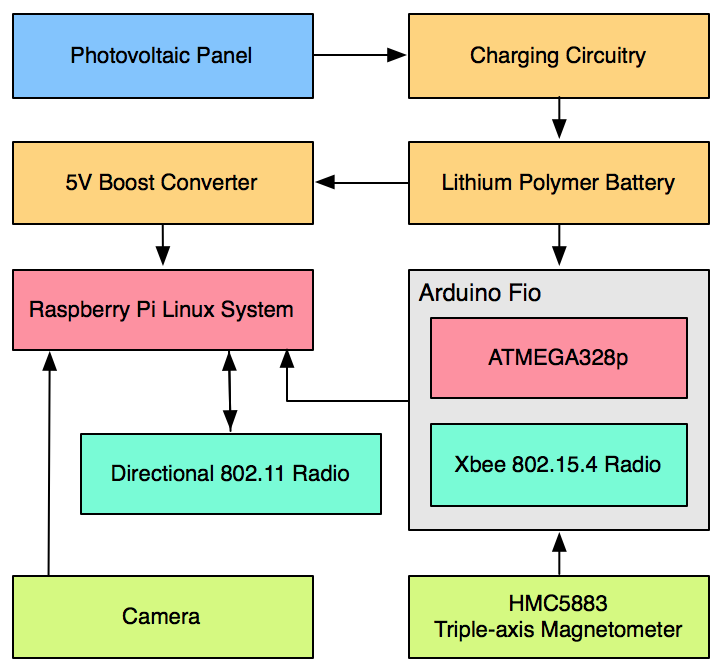
\includegraphics[width=3.5in]{autodetection}
\end{center}
\caption{Automobile Detection Subsystem Architecture}
\end{figure}

The hardware to be used for automobile detection will be contained in the same enclosure as the license plate image acquisition hardware.

The use of a magnetometer ensures that solely automobile and other large vehicles such as motorcycles are detected while pedestrians are ignored.

Work on the automobile detection subsystem will involve a variety of tests and analyses to ensure system and data integrity.


\subsection{License Plate Image Acquisition}
Kevin


\subsection{Central Basestation}
Everyone


\subsection{Server Processing}
Once an image has been determined to contain a license plate, it will be transmitted from the Acquisition Raspberry Pi to a server online via the Central Basestation Pi. The server will then be responsible for using recognition software technology to extract the digits of the license plate from the image. Upon successful completion, the textual representation of the license plate will be stored in a database residing on the server to be later integrated into a front-facing web application.

The subsystem encapsulating server processing will require a review of recognition software and literature. There exists a market for Automatic License Plate Recognition (ALPR) software that relies on Optical Character Recognition (OCR) engines to extract characters. Once an ALPR solution is chosen, it will be necessary to collect a set of test data using the Acquisition Pi to tune the workflow of character extraction. Because the system is being deployed in the metro Denver area, it can be assumed that Colorado plates will make up the majority of license plates the system will detect. Therefore, the last step will be to analyze the accuracy of the ALPR tool on extracting characters from other license plates.

\subsubsection{Review of ALPR Software}
For the scope of this project, three ALPR solutions will be evaluated to determine which is the most suitable for our purposes.

Q-Free Intrada ALPR is a license plate recognition software that offers a C++ API, as well as a cloud-based service. Both the API and cloud requests can be accomplished from a Linux server. Q-Free's software is used in countries around the world for traffic management and toll collection. The wide-ranging geography of its use mean that Intrada ALPR is likely to be reliable and accurate for all types of license plates.

OpenALPR is another C++ library for use with both North American and European plates. This library relies upon two underlying technologies: OpenCV (an open-source computer vision library) and Tesseract OCR (an OCR engine being developed and maintained by Google). The open-source nature of this project make it appealing as it can be immediately integrated without needing to obtain an educational license first.

JavaANPR markets itself as an Automated Number Plate Recognition library using Java's built-in libraries. 

\subsubsection{Collection of Test Data}

\subsubsection{Effect of Different License Plates on OCR Software}



\subsection{Web Application}
Taylor


\subsection{Deployment}
Blah


\section{Summary}
A summary \cite{johnson2012} Talk about the motivation behind this project. Why it is important.


\begin{thebibliography}{99}
\bibitem{stillwell2013} R. Stillwell, A. Wilson ``Magnetometer Parking Sensor'' \emph{EGGN 383 Final Project, Colorado School of Mines}. December 12, 2013

\bibitem{parkingWiki}  ACMx ``Parking Sensor Wiki'' \begin{verbatim}https://github.com/ColoradoSchoolOfMines/parking_sensor/wiki\end{verbatim} % Not sure how to cite this; can someone help?

\bibitem{johnson2012} X. Johnson
\end{thebibliography}





\end{document}  
